
\begin{frame}[fragile]{Le modèle E/A - Concepts avancés}

Cette session présente quelques notions avancées du modèle entité / association

\vfill

\begin{redbullet}
  \item Entités faibles
  \item Associations généralisées
  \item Spécialisation orientée-objet
\end{redbullet}

\vfill
\begin{blocgauche}
\alert{Ces diapositives correspondent au support en ligne disponible sur
le site \url{http://sql.bdpedia.fr/}}
\end{blocgauche}

\end{frame}


\begin{frame}{Entités faibles}

Identification d'une entité \alert{relativement} à une autre entité (toujours
un-à-plusieurs).

\vfill


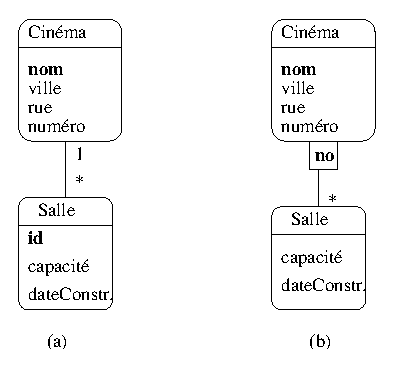
\includegraphics[width=6cm]{../../figures/faible}

\end{frame}


%%%%%%%%
\begin{frame}{Entités faibles: caractéristiques}
La clé de \texttt{Salle} est la paire \texttt{(idCinéma, noSalle)}

\vfill

\begin{redbullet}
  \item quand on insère une salle dans la base, on doit toujours
    l'associer à un cinéma ;
  \item quand un cinéma est détruit, on doit aussi détruire 
    toutes ses salles.
\end{redbullet}

\vfill

On peut très bien utiliser une association classique
\end{frame}


%%%%%%%%
\begin{frame}{Associations généralisées}
Peut-on avoir des associations entre 3, 4 types d'entité ou plus?
\vfill

Oui, mais...

\vfill

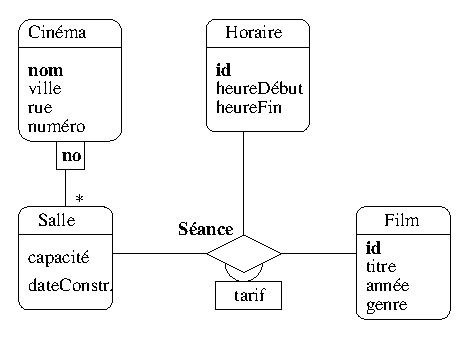
\includegraphics[width=7cm]{../../figures/assoc-tern}

\end{frame}
%%%%%%ù


%%%%%%%%
\begin{frame}{Réification = associations un-à-plusieurs}

On peut toujours se ramener aux associations un-à-plusieurs, et ajouter des contraintes ensuite.


\vfill

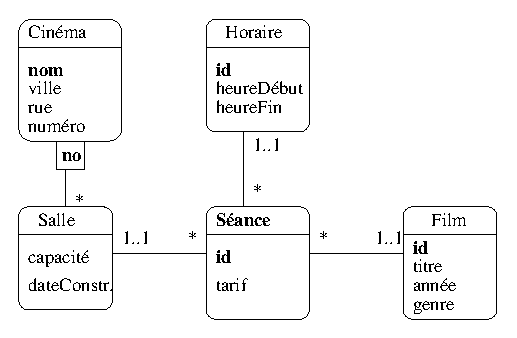
\includegraphics[width=7.5cm]{../../figures/seance}

\end{frame}


%%%%%%%%
\begin{frame}{Spécialisation orientée-objet}

Une structure de modélisation qui va au-delà du relationnel.

\vfill

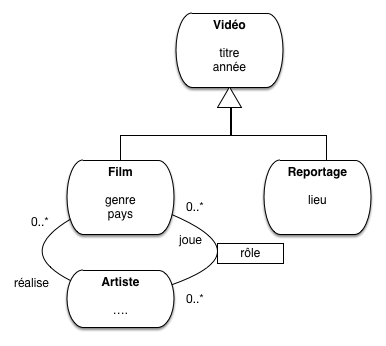
\includegraphics[width=7cm]{../figures-sql/heritage}

\begin{blocgauche}
Cf. support de cours pour cet aspect
\end{blocgauche}
\end{frame}
%%%%%%ù

\begin{frame}{À retenir}

Constructions avancées du modèle E/A: pas indispensables.

\vfill
\begin{redbullet}
  \item les entités faibles apportent une certaine clarification sur la modélisation
  
 \item Les associations entre plus de deux types d'entités sont à éviter
 \item La spécialisation est utile quand on souhaite rendre persistante une application OO
\end{redbullet}
\vfill

Pour ce dernier aspect, voir aussi le \textit{mapping} objet-relationnel,
introduit à la fin du cours
\end{frame}

